\begin{frame}{Mass of \chiboneOneP in $\chib \to \OneS \gamma$ decay}
\begin{center}
\resizebox{.5\textwidth}{!}{
\setlength{\unitlength}{1mm}
\begin{picture}(70,50)
  %
\put(0,0){
  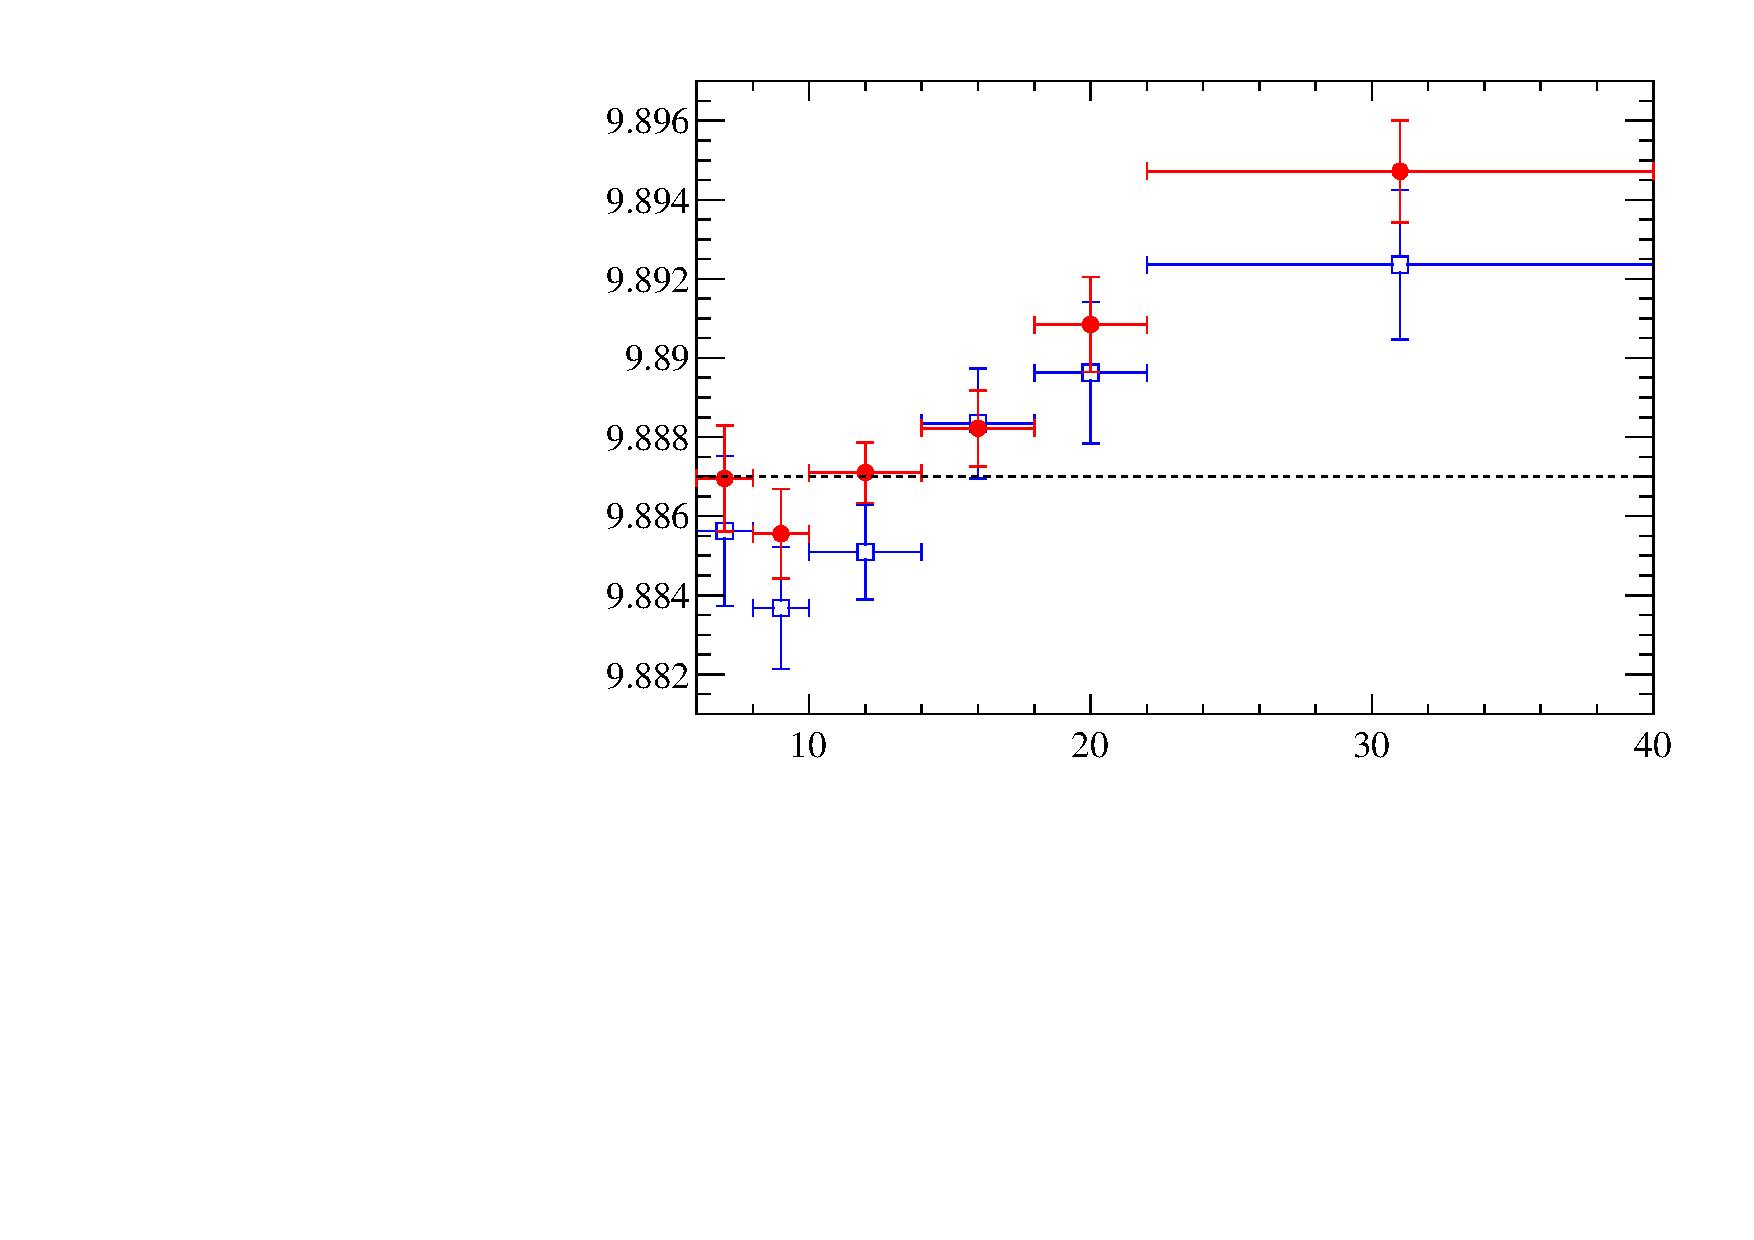
\includegraphics[width=70mm, height=50mm]{chib1s-m/mass1p}
}

\put(27, 15){\textcolor{blue}{\sqs=7\tev}, \textcolor{red}{\sqs=8\tev}}
% \put(27, 40){\textcolor{blue}{\sqs=7\tev}, \textcolor{red}{\sqs=8\tev}}
\put(0,12){\begin{sideways}\chiboneOneP mass \gevcc\end{sideways}}
\put(20,1){$p_T^{\Y1S} \left[\gevc\right]$}
\end{picture}
}
\end{center}
\begin{alertblock}{}
The major cause of  \chiboneOneP mass floating in 10 \mevcc range can be the unknown fraction
between $N_{\chibone}$ and $N_{\chibtwo}$ yields ($\lambda$ parameter). 
We have only theoretical prediction for $\lambda$ value . In this study
$\lambda$ is fixed to 0.5 for all $\chib$ decays.
\end{alertblock}

In the following, this mass was fixed to $9.887\gevcc$  which is the value
measured on the combined 2011 and 2012 datasets. A systematic uncertainty due
to this assumption has been assigned.

\end{frame}